\chapter{K-Dimensional binary search tree}\label{ch:volume_kd}
As we mentioned in Paragraph \ref{sec:hgcal_clustering} in order to form the HGCAL clusters a nearest neighbors search is required. In this chapter we describe one of the known algorithms to efficiently search for nearest neighbors in a large data set.\\
A k-d tree is a data-structure used to partition a k-dimensional space and is a special case of a binary-search tree.

\section{General description of the KD-tree}
A binary tree is a data-structure in which each element of the data-set is hierarchically connected to the other elements which also constitute the so called nodes of the tree.\\
Each node has at most two children, usually referred to as left-child and right-child. Thus from every node of a binary tree develops another sub-tree. The nodes of the tree that does not have any children are called \textit{leaves}.\\
A k-d tree subdivides a k-dimensional space in such a way that the relation between sub-spaces can be represented through a binary tree.
For all intents and purposes of this work, from here on we will consider k=3, therefore always referring to a three-dimensional Cartesian space, however all the following methods and techniques can be extended to any number of dimensions in any basis.
  
\subsection{Building a 3D tree}
The procedure of the tree construction is recursive: a starting point is chosen and it will be called the root of the tree, a plane passing through the root point and orthogonal to one of the axis defines the regions of the two sub-trees children of root, for each of those a new root is chosen between the points of the sub-tree repeating the procedure until all the sub-trees contains no points, those are the leaves of the tree.\\
In order to construct a balanced tree, where each sub-tree of a given level contains the same amount of points, there are two requirements: the first is that the subdivision must be performed cycling along the Cartesian axes, so if the first splitting is done by a plane orthogonal to $x$, the second will be done with respect to $y$, the third to $z$, the fourth again through $x$ and so on until all the leaves are created.\\
The second requirement is to choose the root of each sub-tree in such a way that both of its sons will contains the same amount of points (with the exception of one point in case of odd numbering that will conventionally be assigned to the left son). To achieve that all the points of a sub-tree are sorted according to their coordinate in the axis along which the sub-tree will be divided, the root will be the middle point defined by that with as many points preceding as many following it.\\
The relations between each node and its sons is then recorded and the procedure stops when all the elements of the set are also nodes of the tree.

\subsection{Traversing a 3D tree}
The purpose of creating a binary tree data-structure is to greatly reduce the number of comparisons required to search a given point -and/or its neighbors- in the whole set.\\
The procedure is again recursive: consider for instance the search of the nearest neighbor of an arbitrary input point among the points of the data set: using the same axes-cycling described in the building evaluate if the point is smaller or greater than the root along the axis picked. If it is smaller the search will continue on the left-child of the root, otherwise on the right-child. The second step is to compare the point to be searched with the node child of root chosen by the previous step, again comparing it along the next axis in the cycle (always maintaining the same axis-cycling order used in the construction). The procedure continues until a node without any child is reached: a leaf, which is the closest point of the set to the input point.\\
Considering the procedure described above it is clear that this type of search discards half of the points of the data set at each step. It is therefore expected that the complexity of this search is $\mathcal{O}(\log{} n)$ where simply comparing the input point to all the points in the data set would have complexity $\mathcal{O}(n)$ where $n$ is the total number of points in the data set.\\
The nearest neighbors search is just a slight variation of the above described procedure that is all the points in the data-set contained in a volume centered around an input point. The search procedure for the ``box" would be similar to the one explained for the single nearest neighbor, the only caveat being that the box can be not only ``left" or ``right" of a given node but also intersecting it. In the case of intersection both child of the node are considered for further searching. The complexity of this case has to be worse than that of a single point, in particular has been demonstrated \cite{worst-case-search} that the worse-case run-time is $\mathcal{O}(k n ^{1 - {1\over k}})$ for a k-dimensional tree of $n$ elements.

\section{Volume kd-tree}
A possible implementation of the above-described algorithm uses as tree nodes volumes in the 3D space that splits the space in which the data set points lies. Therefore the root node will be the smallest volume containing all the data set points, its children will be each half of the root, their children a quarter and so on until the leaves are created.\\
The advantage of such an implementation is that every sub-tree describes the 3D region containing all of its elements, therefore, when performing a nearest neighbors search, the search box is compared with volumes of decreasing size (the nodes of the tree) up to a point where the search box fully encloses a node: at this stage the search procedure can halt without reaching the leaves, since all the nearest neighbors are the points of the sub-tree reached, which are known because of the tree structure.\\

Following we will describe the specific implementation of the volume kd-tree we developed for this work.
\subsection{Build}
As mentioned above this implementation uses volumes as nodes of the tree which, being \textit{rectangular cuboids} in a 3D Cartesian space, can be described by only two triplets: the coordinates of the \textit{minimum} and the \textit{maximum} vertices. Where the minimum vertex is defined to be the one where each coordinate is the smallest, while the maximum the one with the greatest coordinates. This method of describing the tree nodes will benefit both the memory footprint of the tree and the process of comparing the search box position with respect to the tree nodes.\\
The building is performed similarly to what described in the generic kd-tree with the exception that for every iteration splitting in half the volume, two new volumes are created (the children).\\
For this implementation the splitting plane passes through the median point among the set contained in that sub-tree, which is found by using the \textit{tbb::parallel\_sort} method provided by Intel's Threading Building Blocks library \cite{intel_tbb} to parallelize the sorting on the CPU when a multi-core processor is available.\\
The left-child is then defined to have the same minimum vertex of its parent, while the maximum is the same of the parent except for one coordinate: the one along the axis of the splitting. That coordinate is then the same of the median point found by sorting the set. The right-child is built similarly by substituting the coordinate in the minimum vertex. The procedure is described by algorithm \ref{volume_kdtree_build}.\\

\begin{algorithm}
\caption{The build of the volume 3D-tree}
\label{volume_kdtree_build}
\begin{algorithmic}
\State BuildKDTree(totalNuberOfPoints, allPoints, 0) \Comment First call
\Procedure{BuildKDTree}{numberOfPoints, points, depth}
  \State axis $\gets$ depth $\bmod$ 3 \Comment 0 = $x$, 1 = $y$, 2 = $z$
  \State medianValue $\gets$ ceil(numberOfPoints / 2) \Comment The index of the median point
  \State \textbf{sort}(points, axis) \Comment Parallel sort of the input point along axis
  \State newCoordinate $\gets$ points[medianValue][axis]
  \State leftChild $\gets$ newCoordinate
  \State rightChild $\gets$ newCoordinate
  \State tree $\gets$ leftChild
  \State tree $\gets$ rightChild
  \If{(remainderPoints $>$ 0)}
  \State \textbf{return} \small{BuildKDTree(ceil(numberOfPoints/2), remainderPoints, depth+1)}
  \EndIf
\EndProcedure
\end{algorithmic}
\end{algorithm}

\subsection{Range search}
The search for the nearest neighbors of a given point begins by defining a region of the space to search the neighbors in.
The ``search box" is defined by the pair of coordinates describing a volume enclosing the point for which the neighbors are searched. The search is again recursive, it starts from the tree's root node. The minimum and maximum coordinates of the search box along the root's splitting axis are compared to the minimum and maximum coordinates of the children nodes along the same axis where the division took place at the construction phase. As usual only the coordinates along the axis determined by the depth of the tree are considered: if both coordinates of the search box are within those of the left-child  the search continues there, if both are within those of the right child the search proceeds there and if the search box coordinates are across both children the search proceeds on both of those nodes. In the case where a child's coordinates are within those of the search box then all the points of the child are considered as nearest neighbors and the search stops. Otherwise the search stops when a leaf is reached.\\
The whole procedure is illustrated in algorithm \ref{volume_kdtree_search}.\\
\begin{algorithm}
\caption{The build of the volume 3D-tree}
\label{volume_kdtree_search}
\begin{algorithmic}
\State SearchKDTree(searchBox, root, 0) \Comment First call
\Procedure{SearchKDTree}{searchVolume, nodeToSearch, depth}
  \If {(nodeToSearch is a leaf)}
    \State \textbf{return} node[thisPoint]
  \EndIf
  \State axis $\gets$ depth $\bmod$ 3
  \State searchBoxMin $\gets$ searchBox[minimumVertex][axis]
  \State searchBoxMax $\gets$ searchBox[maximumVertex][axis]
  \State nodeMin $\gets$ nodeToSearch[minimumVertex][axis]
  \State nodeMax $\gets$ nodeToSearch[maximumVertex][axis]
  \If{ (searchBoxMin $\leqslant$ nodeMin \&\& searchBoxMax $\geqslant$ nodeMax)} 
  \State \textbf{return} node[points] \Comment save all node's points as NN
  \Else
  	\If{ searchBoxMin $\leqslant$ nodeMin}
  	  \State \textbf{return} SearchKDTree(searchVolume, leftChild, depth + 1)
  	\EndIf
  	\If{ searchBoxMax $\geqslant$ nodeMax}
 	  \State \textbf{return} SearchKDTree(searchVolume, rightChild, depth + 1)
	\EndIf
  \EndIf
\EndProcedure
\end{algorithmic}
\end{algorithm}

\section{Validation}
We implemented the algorithm described above in \CC\ and developed the following method to validate the results of the searches performed with the volume kd-tree.\\
Using the Standard Template Library (STL) pseudo-random uniform generator defined by the \CC 11 ISO standard we place a number of points ranging from $2 \times 10^{4}$ to $3 \times 10^{5}$ in a cube of side 100 arbitrary units (a.u.). We build a volume tree with the generated points and for each of the points we perform a range search for a cube of side ranging from 1.0 a.u to 10.0 a.u. centered on the point for which we want to search the nearest neighbors and the results are recorded.\\
As comparison we perform again the nearest neighbors search through a method called \textit{naive} since it is the simplest possible way to perform such a search: for each search box every single point of the data set is checked: if it lies inside the box it is recorded. It is also clear that the naive method is very inefficient having complexity $\mathcal{O}(n^{2})$ when searching the nearest neighbors of all $n$ points. However it is a simple and reliable method to validate less intuitive algorithms and we used it extensively as a validation tool throughout this work.\\
The data set random generation is executed for different numbers of data set points and different sizes of the search boxes and both searches -naive and kd-tree- performed, the results of the two methods are then compared for each generation and only when they are always identical the kd-tree range search algorithm is declared valid.

\section{GPU porting}
The GPU architecture we described in Chapter \ref{ch:gpu} requires some adaptations of the code to best perform on this device. We list here the most relevant:
\begin{itemize}
\item The specific parts of code that runs on the GPU must be CUDA-compliant e.g. STL containers must be avoided and only some \CC\ constructs can be used.
\item Input data must be moved on the GPU device and must have the smallest possible byte size to avoid that the data transfer rate becomes a significant bottle-neck.
\item Several processes must run simultaneously as, ideally, all the GPU computational cores must be used at the same time.
\item Output data must be moved back from the GPU device to the host machine and the size of the output data has to be known.
\end{itemize}
We first attempted to perform the tree construction on the GPU device, should that performed well not only we would have exploited the GPU computation for this part of the algorithm too, but we would have had the tree saved on the GPU memory without needing to move it. Unfortunately it became soon apparent that it wasn't possible to build the tree in a way that employed all the GPU cores at the same time and the performance were worse than those obtained on the CPU.\\
The all nearest neighbors search is much simpler to parallelize in order to fill up the GPU cores: by assigning a search box to each GPU core they can all run simultaneously and independently. Therefore once the tree is built on the host machine there are two inputs that needs to be loaded onto the GPU memory: the tree itself, which can be expressed as an array of pair of vertices of $n$ elements for $n$ data set points and the search boxes which again is an array of pair of vertices of $n$ elements.\\
The search code itself is the very same that runs sequentially on the CPU, however the code generates one CUDA thread for every search box to be found, then the GPU device scheduler takes care of executing each of those threads on all the available GPU cores, reaching the concurrential execution desired.\\
The output result is a single array where the indices of the nearest neighbors are recorded. As mentioned before the size of this array must be known before the search is performed which implies the need of an assumption on the number of nearest neighbors found for each search box. In the case of the uniform random generation of $N_{total}$ points in a volume $\mathcal{V}$ we evaluate the statistical average density of nearest neighbors found in a search box of volume $\mathcal{V_s}$ and we double the average number of points per search volume to take into account the statistical variance.
\begin{center}
\begin{equation}
N\!N_{max} =  N_{total} \cdot \dfrac{\mathcal{V_s}}{\mathcal{V}} \cdot 2.0
\end{equation}
\end{center}

Thus the array size is $N_{total} \cdot N\!N_{max}$, however most of the times the number of actual NN found is lower than the maximum allowed, therefore a trailing $-1$ is used to instruct the code reading the output that there are not any more nearest neighbors for that search box.\\
The formula described above clearly cannot be applied to real-world applications where the distribution of points is not uniform, therefore other assumptions must be evaluated.\\

\section{Performance analysis}
The assessment of the performance of the GPU algorithm is done by comparison with the same code running sequentially on the CPU.\\
The two search methods runs on the exact same points, generated by a uniform random distribution, similarly to what is done for the validation. Likewise the measurements are repeated for a series of numbers of initial points, ranging from  $2 \times 10^{4}$ to $3.5 \times 10^{5}$. The volume in which the points are generated is a cube of side 100.0 a.u. while the reference search box is a cube of side 4.0 a.u.\\
The computational time spent in each search is evaluated through \textit{cudaEvent} provided by the CUDA libraries which provides a time resolution of $\sim 0.5\unit{ms}$. The tests are performed on the benchmark machine described in Paragraph \ref{sec:benchmark}.\\
Table \ref{volume_kd_tree_tab} reports some selected results, while Figure \ref{volume_kdtree_plot} shows the timing in a logarithmic scale for all the tests performed, lastly Figure \ref{volume_kdtree_speedup} shows the speedup between the GPU-parallel and the CPU-sequential codes.\\

\begin{center}
\begin{table}[h]
\begin{tabular}{ c || r r r r r r r }
Points ($10^{3}$) & 50 & 100 & 150 & 200 & 250 & 300 & 350 \\
\hline
CPU ($\unit{ms}$) & 163.8 & 528.4 & 1186 & 2234 & 3091 & 4225 & 5501 \\
GPU ($\unit{ms}$) & 75.3 & 229.7 & 430.5 & 681.8 & 953.9 & 1281 & 1639 \\
\end{tabular}
\caption{Volume Kd-tree selected search times for CPU sequential and GPU parallel code}
\label{volume_kd_tree_tab}
\end{table}
\end{center}

\begin{figure}
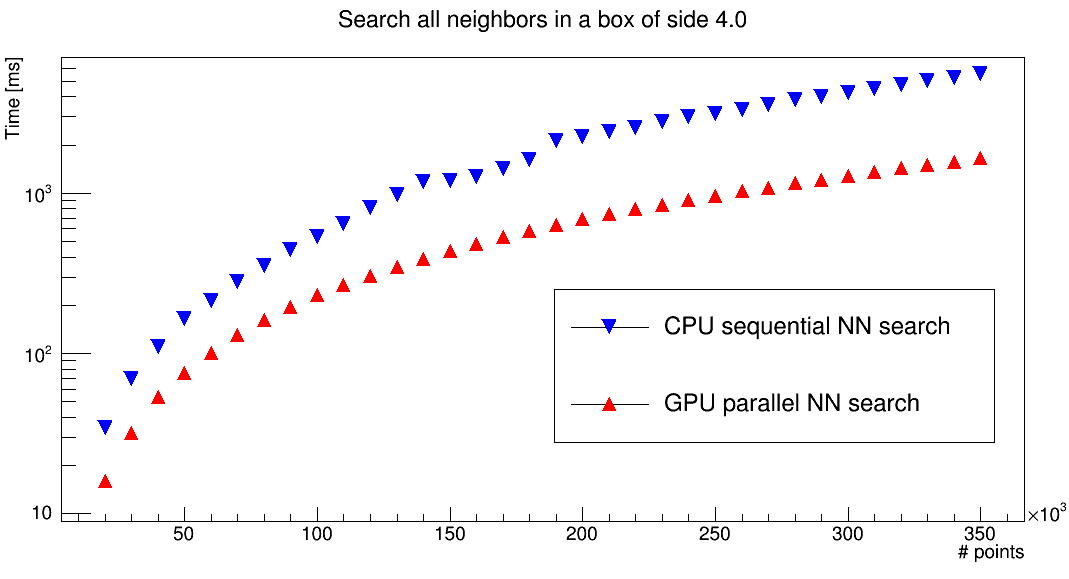
\includegraphics[width=\textwidth]{volumeKdPlot/volumeKdTree.png}
\caption{Volume Kd-tree search times for CPU sequential and GPU parallel code}
\label{volume_kdtree_plot}
\end{figure}

\begin{figure}
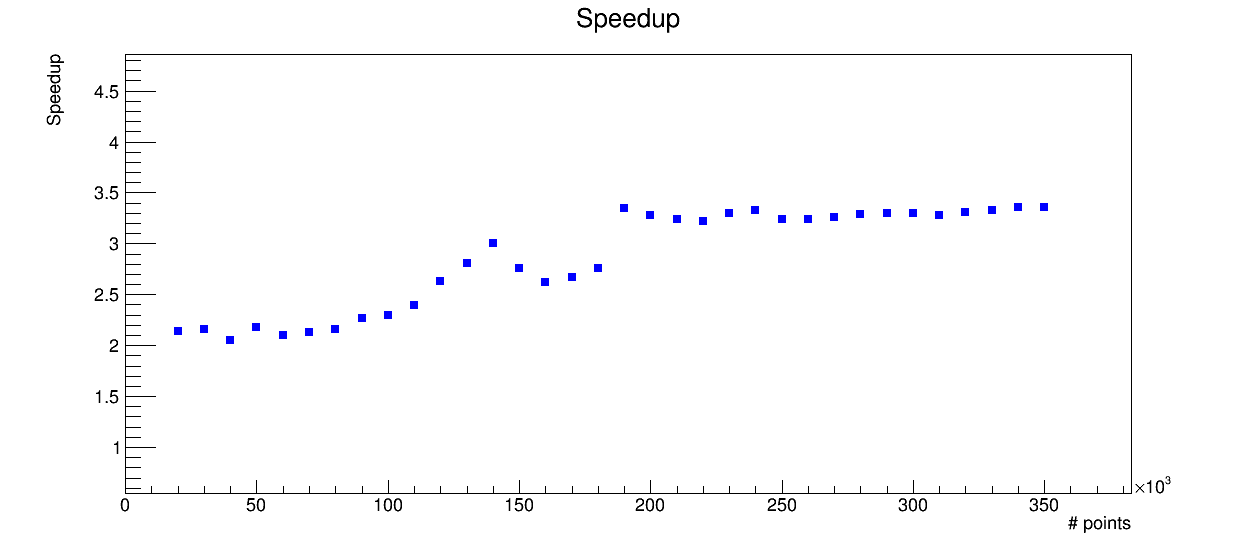
\includegraphics[width=\textwidth]{volumeKdPlot/volumeKdSpeedup.png}
\caption{Volume Kd-tree speedup between CPU sequential and GPU parallel code}
\label{volume_kdtree_speedup}
\end{figure}
\newpage

\section{Algorithm assessment}
The first thing to note in Figure \ref{volume_kdtree_plot} is the relative performance of the two methods for the lowest number of points used: in that regime the GPU parallel code is still faster than the sequential one, implying that the data transfer time needed to load the input and unload the output to/from the GPU also scales with the number of points and does not add a significative fixed time contribution to the process. This is an important feature as the algorithm must perform well in all the ranges at which it can be operated.\\
The CPU sequential timings, however, are not very encouraging requiring up to $5.5 \unit{s}$ to process the highest number of points. This result is well outside of the requirements imposed by the Phase 2 of LHC.\\
According to Figure \ref{volume_kdtree_speedup} the parallel GPU code is always faster than its sequential counterpart by a factor $\sim 2$ to $\sim 3.5$, gaining performance as the number of points to be processed increases. While this is a desired feature of the parallel code, implying that it scales well with the increase of points, the GPU code is also too slow for the requirements.\\
Further analysis of the code, performed at runtime, reveals two major issues with the algorithm developed for the range search of the volume kd-tree, regardless of its parallel or sequential implementation. The first one is caused by the way we save the tree nodes in the array: as they are not assigned to a specific place, but rather just to the last available place, at every recursion the node visited is asked for the index of its sons. The process of accessing the memory to read the indices of the node's sons is relatively expensive and it adds up quickly when repeated millions of times in all the recursions.\\
The second issue derives from a missed performance gain opportunity: despite we designed the volume kd-tree in a way that could quickly return sets of near points when the search box would contain an entire node, analysing the code running with the conditions described above, revealed that this feature is seldomly used if ever. As a matter of fact the size chosen for the volume we distribute the initial data set and the size of the search box we used for the testing are such that when the search box contains a node that is not a leaf the node is still too small compared to the total volume and contains few points, making the contribution of this feature negligible.\\
As a result of the above consideration we determine that the volume kd-tree is not the best suited data-structure for the geometry and times constraints that this work aims to tackle. The following chapter presents a different implementation of a kd-tree where the above issues has been solved.\\




